\documentclass[crop=false,class=mitthesis,oneside,font=12pt]{standalone}
%----------------------------Preamble-------------------------------%
\usepackage{amsmath}
%\newcommand{\angstrom}{\textup{\AA}}
\usepackage{microtype}
\usepackage{graphicx}
\graphicspath{{./images/}}
%\usepackage{multirow}
\usepackage{rotating}
\usepackage{natbib}
\usepackage{url}
\usepackage{booktabs}
\usepackage{makecell}
\usepackage{graphicx, float}            % Graphics/Images.
\usepackage{pgfplots, tikz}             % Drawing/graphing tools.
\usetikzlibrary{
    calc,                   % Calculating right angles and more.
    angles,                 % Drawing angles within triangles.
    arrows.meta,            % Latex and Stealth arrows.
    quotes,                 % Adding labels to angles.
    positioning,            % Relative positioning of nodes.
    decorations.markings,   % Adding arrows in the middle of a line.
    patterns,
    arrows,
    shapes,
    shapes.geometric,
    cd,
    hobby,
    babel
}                                       % Libraries for tikz.
\pgfplotsset{compat=1.9}                % Version of pgfplots.
\usepackage[]{pdfpages}
% for line numbers comment the next two lines before final submission
\usepackage{lineno}
\linenumbers*[1]
% use fancyhdr, to enable page style stuff (below)
\usepackage{fancyhdr}
\setlength{\headheight}{15.2pt}
\renewcommand{\headrulewidth}{0pt}

\pagestyle{plain}
\usepackage{import}                     % Import external files.
\usepackage[subpreambles=false]{standalone}      % Complileable sub files.
\begin{document}
\chapter{Conclusion and Recommendation}

\section{How well can multi-spectral measurement infer Energetics of Auroral Emission ?}
An aurora was observed over Lowell, MA on 22–23 June, 2015 and observed by HiT\&MIS simultaneously in red, green and blue lines.  Energies and fluxes of precipitating electrons were derived based on the brightness measurements of these emissions. The electron energies and energy fluxes as a function of time and look direction were derived by nonlinear minimization of model predictions with respect to the measurements. Three different methods were compared; in the first two methods, the modeled brightnesses and brightness ratios, respectively, we constrained with measurements to simultaneously derive energies and fluxes. Then, a hybrid method where the individual modeled brightness ratios were constrained with measurements to derive energies and then  modeled brightnesses were constrained with measurements to derive fluxes.  The hybrid method is similar to methods that have been used before and thus was used as validation for the other two methods. It was found that the brightness ratio method is not sensitive to the energies and fluxes simultaneously. However, energies and fluxes derived using the brightness method and the hybrid methods were comparable.  Thus, it is concluded that multi-spectral imaging can be used to simultaneously derive energy and flux of auroral electron precipitation by constraining at-least three auroral brightnesses with model estimates.

% Derived energy, assuming Maxwellian distribution, during this storm ranged from 109 to 262 eV and the total energy flux ranged from 0.8 to 2.2 ergs cm$^{−2}$ s$^{−1}$.
% \section{Problem Statement}
% How well can multi spectral measurements be used to quantitatively confine the energy inputted into the atmosphere during geomagnetically active times.

% \section{Approach}
\section{Was the total solar eclipse of August 21, 2017 responsible for the Traveling Ionospheric Disturbances observed in airglow observations ?}
Wave-like structures in the upper atmospheric nightglow brightness were observed on the night of August 22, 2017, approximately 8 hours following a total solar eclipse. These wavelike perturbations are signatures of  Atmospheric Gravity Waves (AGWs) and associated Traveling Ionospheric Disturbances (TIDs). Observations were made in the red line and the green line from Carbondale, IL, from around 2--10 UTC on August 22, 2017. Based on the wavelet analyses, the dominant time period in both the red and green line was around 1.5 hours. Differential Total Electron Content (DTEC) data obtained from GPS TEC measurements at Carbondale, IL, and ionospheric parameters from digisonde measurements at Idaho National Laboratory and Millstone Hill showed a similar dominant time period. Vertical (24 $\pm$7 m/s) and horizontal (154 $\pm$ 44 m/s) phase velocities of the TIDs are estimated using cross-correlation analysis between red and green brightness profiles and TEC measurements at two different locations, respectively. Based on these observations and their correlation with geomagnetic indices, the TIDs appear to be associated with geomagnetic disturbances. In addition, by modeling the Ionosphere-Thermosphere (IT) system's response to the eclipse, it is seen that preconditioning of the IT system due to the eclipse enhanced O/N$_2$ ratio and the electron density (N$_e$) at 250 km. Thus, while the eclipse did seem to enhanced the observed brightness, the observed brightness perturbations (and associated AGWs) seem to have been caused by geomagnetic disturbances.


\section{Recommendations} \label{sec:recommendations}

During the day, there is a need to subtract out the solar background continuum which is a few orders of magnitude brighter than the underlying spectrum. Thus, high-resolution imaging (Full Width Half Max (FWHM)$<$0.01 nm at red line \citep{hitmis}) is needed to disperse the light so that it can be matched with a reference solar spectrum and subtracted to extract the underlying spectra. See Figure \ref{fig:mise}, to see the daytime spectra extraction process and Figure \ref{fig:mise_b} for daytime brightnesses measured using the daytime spectra. However, in its current setup HiT\&MIS's is resolution limited to extract such spectra (FWHM$\sim$ 0.1 nm). Thus, by using smaller slit width or using gratings with higher groove density, the former of which requires minimal change to the current setup daytime spectra extraction is possible. 
\begin{figure}[H]
	\centering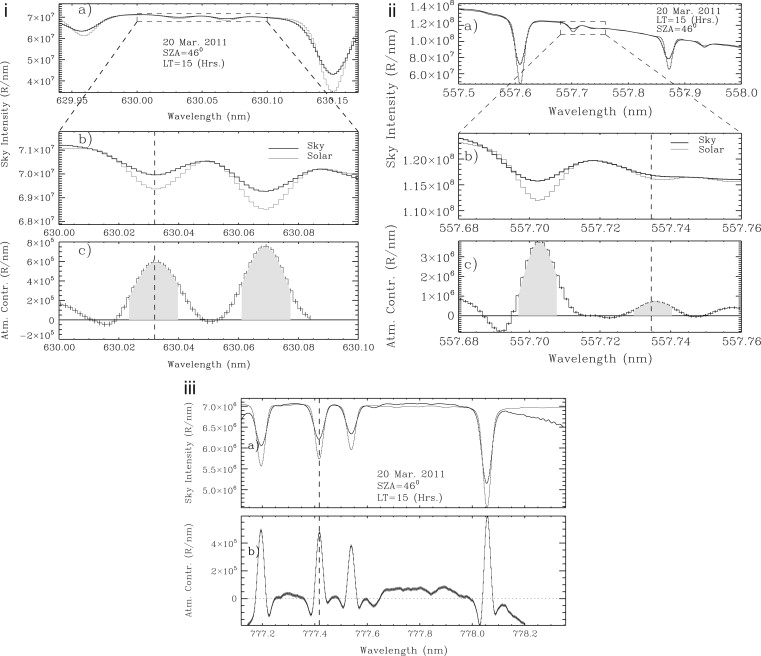
\includegraphics[width=25pc]{mise_day.jpg}
	\caption{GLOW model blue line brightnesses with and without the resonance fluorescence contribution.}
	\label{fig:mise}
\end{figure}
\begin{figure}[H]
	\centering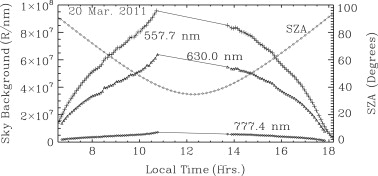
\includegraphics[width=25pc]{mise_brg.jpg}
	\caption{GLOW model blue line brightnesses with and without the resonance fluorescence contribution.}
	\label{fig:mise_b}
\end{figure}


\end{document}